\chapter{Literature Review}\label{litrev}

\section{Intrumentation}

To observe FRBs, both single dish telescopes and interferometry techniques are used. Single dishes like the Parkes Telescope, Green Bank Telescope and the Five-hundred-meter Aperture Spherical Telescope (FAST) are used due to their high sensitivity, allowing for accurate flux readings, but suffer from large location uncertainty \cite{Keane2016}. On the other hand, interferometry allows for higher resolution and are much more versatile as these can perform fly's eye survey \cite{Shannon2018} allowing for a much higher detection area. However, they are computationally expensive and inefficient for real time tracking. In practice, both are used in FRB detection to utilise their advantages e.g. single dishes would first detect the FRB, and its source is localized using interferometry techniques \cite{Marcote2020}. 

FRB searching or observations are usually done blind where radio telescopes would observe a large portion of the sky over a certain period of time \cite{Keane2017}. However, recently some observations are made near hosts of soft gamma-ray bursts  i.e. large bursts of gamma rays and X-rays, which are also known as soft gamma repeaters or SGR \cite{Madison2019, Katz2020}. This is because SGRs have been conjectured to be from magnetars, and as stated earlier, are also one of the leading hypothesis for FRBs. 

%The two instrumentation challenges in FRB detections are RFI mitigation and dedispersion. Strong RFI are removed by masking contaminated frequency channels, whereas weaker RFI are removed by subtracting the interference modulation spectrum i.e. Fourier transform of zero-DM spectrum \cite{ransompresto,Kocz2010} or using zero-DM matched filter \cite{Men2019}. Then, for a new FRB, the DM has to be measured in order for the peak to be dedispersed i.e. remove time delay in the signal between frequencies. This is done by testing for all DMs while maximizing the SNR and is computationally heavy, requiring techniques such as incoherent dedispersion, transient search algorithms, tree dedispersion \cite{Barsdell2012}, and GPU parallelization \cite{Magro2011}.

\section{Data Analysis}

Previously, FRB data from radio telescopes are detected and/or analysed using pulsar signal processing programs such as \texttt{SIGPROC} and \texttt{PRESTO}, based on methods that search for new pulsar candidates. Currently, there are many FRB searching softwares such as HEIMDALL and BEAR, and they are mainly based on the matched filter, quoted as the \textit{most powerful statistics} for detecting signals with a priori waveform \cite{vain1970extraction} and are performed based on the methods underlined in \citeNP{Cordes2003}. Most FRB data analysis programs have a similar flow, starting with the input which is a binary data file called filterbanks \cite{Lorimersigproc}. The data is then passed through radio frequency interference (RFI) removal/mitigation. Strong RFI are removed by masking contaminated frequency channels, whereas weaker RFI are removed by subtracting the interference modulation spectrum i.e. Fourier transform of zero-DM spectrum \cite{ransompresto,Kocz2010} or using zero-DM matched filter \cite{Men2019}. Then, the program performs dedispersion at different DMs i.e. removing the dispersion delay, using various optimization algorithms such as the tree algorithm, subband dedispersion and/or using CPU or GPU parallelization \cite{Magro2011,Barsdell2012}. The program then applies the matched filter to the dedispersed data, for which the peaks are reported as FRB candidates. The candidates are then passed through candidate grouping i.e. clustering of candidates of the same event \cite{Pang2018}, and through filters corresponding to parameters such as their DM (only signals with large DMs are considered as FRBs), SNR (only signals with SNR above a certain threshold), pulse width, and for multi-beam receivers, the number of beams detected (large number of detection beams may be due to terrestrial sources). Finally, the results are manually examined to confirm the signal is an FRB i.e. depending on the presence of the dispersive sweep in the non-dedispersed data \cite{Rane2015}.

\begin{figure}
    \centering
    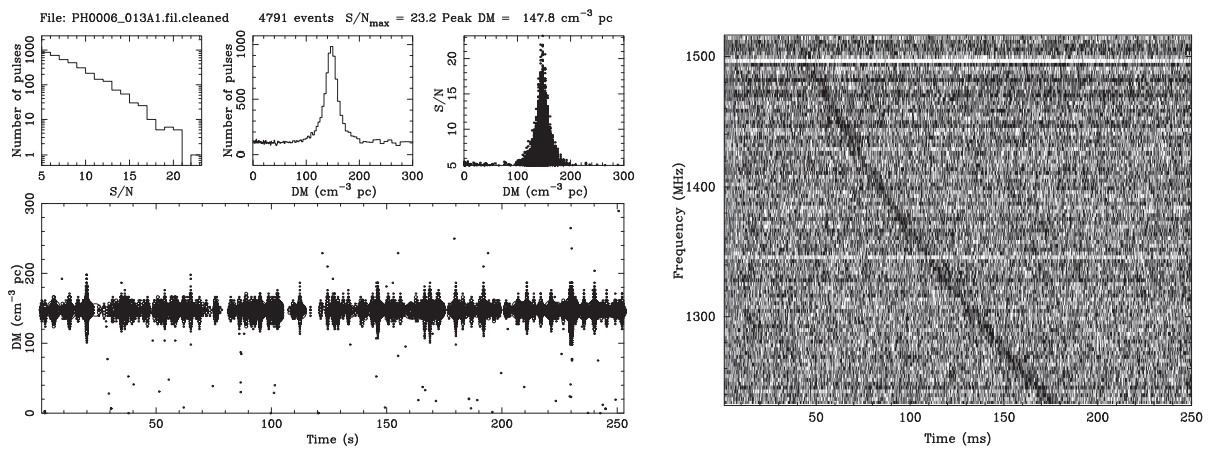
\includegraphics[width=\textwidth]{Images/presto.jpg}
    \caption[PRESTO's pulse processing pipeline output]{Output of PRESTO's pulse processing pipeline for single pulse from PSR J0837-4135. The non-dedispersed spectrum (right plot) displays a noticeable dispersive sweep, corresponding to a large DM \protect\cite{Rane2015}.}
    \label{fig:presto}
\end{figure}

\section{Pipelines}

%To analyse radio telescope signals from FRBs, pulsar signal processing programs such as \texttt{SIGPROC}\footnote{SIGPROC: \url{http://sigproc.sourceforge.net/}} and \texttt{PRESTO}\footnote{PRESTO: \url{https://github.com/scottransom/presto}} are used. The raw telescope data is in the form of filterbanks. First order in data analysis is to perform RFI removal \cite{Lorimer2007}. Then, dedispersion is performed at different DMs, and here DM search algorithms such as the tree algorithm and bonsai algorithms are used \cite{ransompresto}. The program then searches for pulses, and then passed through filters corresponding to parameters such as their DM (only signals with a large DMs are considered as FRBs), SNR (only signals with SNR above a certain threshold), pulse width, or for multi-beam receivers, number of beams detected. Finally, the results are folded and manually examined to confirm the signal is an FRB i.e. depending on the presence of the dispersive sweep in the non-dedispersed data \cite{Rane2015}. 

With the ever increasing number of telescopes used to observe FRBs, the data obtained exponentially increases, presenting researchers with a `data avalanche'. Therefore, to quickly filter through the data, pipelines i.e. automatic sequencing of programs, are used to detect and analyze FRBs in telescope data, outputting FRB candidates \cite{Petroff_Hessels_Lorimer_2019}. Along with the previously stated processes, pipelines also include DM refining using repetitive dedispersion and SNR search, as well as localization using SNR sky maps. Pipelines are often independently developed for specific telescopes to efficiently make use of their corresponding parameters. Examples of FRB detection/analysis pipelines include:
\begin{itemize}
    \item Westerbork Telescope: AMBER which utilizes multi-core GPU computation and real time detection \cite{Sclocco2020}.
    \item CHIME/FRB: `bonsai' algorithm i.e. a more efficient tree dedispersion algorithm, and Apache Airflow and Docker based analysis pipeline to automatically schedule processes \cite{Chime2018, Michilli2021}.
    \item Arecibo Telescope: PALFA Single-pulse Pipeline based on PRESTO's \texttt{single pulse search} \cite{Patel2018}.
    \item MeerKAT: MeerTRAP which uses both coherent mode where multiple beams are interfered for localization and incoherent mode where beams are summed over for a large field-of-view \cite{Sanidas2017}.
    \item ASKAP: CRAFT which utilizes fly's eye survey using each dish independently, and the FREDDA algorithm \cite{James2019}.
\end{itemize}